\documentclass[letterpaper,12pt]{article}
\usepackage{amsmath}  % improve math presentation
\usepackage{graphicx} % takes care of graphic including machinery
\usepackage{mathrsfs}


\usepackage[final]{hyperref} % adds hyper links inside the generated pdf file
\hypersetup{
	colorlinks=true,       % false: boxed links; true: colored links
	linkcolor=blue,        % color of internal links
	citecolor=blue,        % color of links to bibliography
	filecolor=magenta,     % color of file links
	urlcolor=blue         
}

\title{Eighth Assignment for Computational Physics}
\date{\today}
\author{Xinyu Liu}


\begin{document}
\maketitle
\tableofcontents

\newpage

\section{My Github Page URL}
\url{https://github.com/rising1227/phys-ga2000}

\section{Logistic regression}

In this problem we use a logistic model to fit the data, between ages and whether they know a certain phrase. In the code we first define our logistic model as a function. Then a loss function is defined as:

\begin{equation}
    L = -p*log(0.01 + 0.99*q) -(1-p)*log(1 - 0.99*q) + 0.0001*(\beta_0^2 + \beta_1^2)
\end{equation}

Where p is the real data and q is the predicted probability given by logistic model. We've modified the common negative log likelihood function by a little bit to avoid doing log for a value very close to 0. We also added a regularization term to avoid very large parameters.

After defining a loss function, we use a optimizor(optimize.minimize) to minimize this loss function and find the best fit parameter. In this process we use jax diff function to do automatic differentiation. We found that:

\begin{itemize}
    \item The maximum likelihood values is:$\beta_0 = -5.83248073$, $\beta_1 = 0.11416234$
    \item The error for $\beta_0$ and $\beta_1$ is: [1.162193   0.02321067]
    \item The covariance matrice for $\beta_0$ and $\beta_1$ is:  [[ 1.3506925e+00, -2.5923811e-02], [-2.5923807e-02, 5.3873518e-04]]
\end{itemize}

We can plot the real data and the logistic regression result in a same plot, here's the result.

\begin{table}[!h]
    \centering
    \caption{Real data and the logistic regression of the result}
    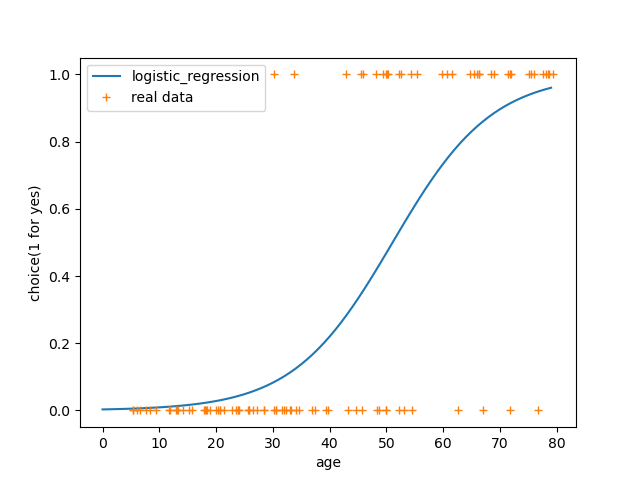
\includegraphics[width=11cm]{8-1-1.png}
\end{table}%
\newpage

The result make sense to me. It shows that this phrase is more common in aged people. People with higher age has higher probability to know this phrase.

\section{Newman 7.3: Fourier transformation for musical instrument}

We use numpy to read the txt file into numpy array. This is plotted as follows:

\begin{table}[!h]
    \centering
    \caption{Waveform for piano}
    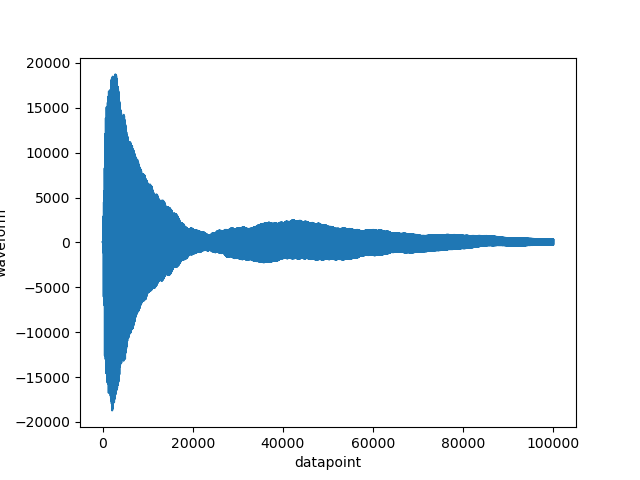
\includegraphics[width=11cm]{8-2-1.png}
\end{table}%

\begin{table}[!h]
    \centering
    \caption{Waveform for trumpet}
    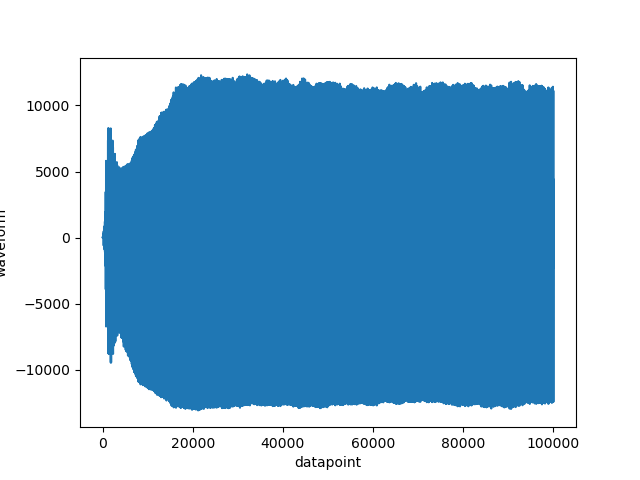
\includegraphics[width=11cm]{8-2-2.png}
\end{table}%

\newpage
In order to see some detail of the waveform, we plotted the number 5000-7000 data in the array(there's a total of $10^5$ data point)

\begin{table}[!h]
    \centering
    \caption{Zoomed waveform for piano}
    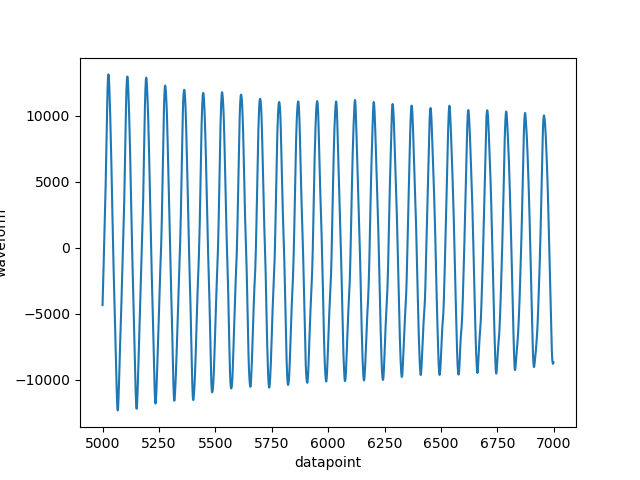
\includegraphics[width=10cm]{8-2-3.png}
\end{table}%

\begin{table}[!h]
    \centering
    \caption{Zoomed waveform for trumpet}
    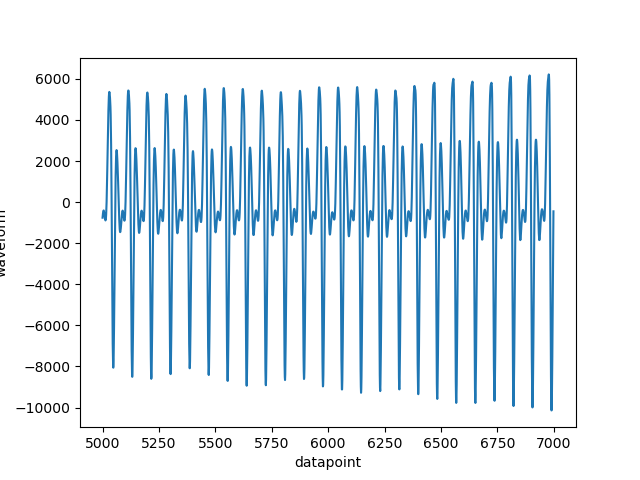
\includegraphics[width=10cm]{8-2-4.png}
\end{table}%
\newpage
We then do the FFT for the waveform.

\begin{table}[!h]
    \centering
    \caption{Fourier coefficient for piano waveform}
    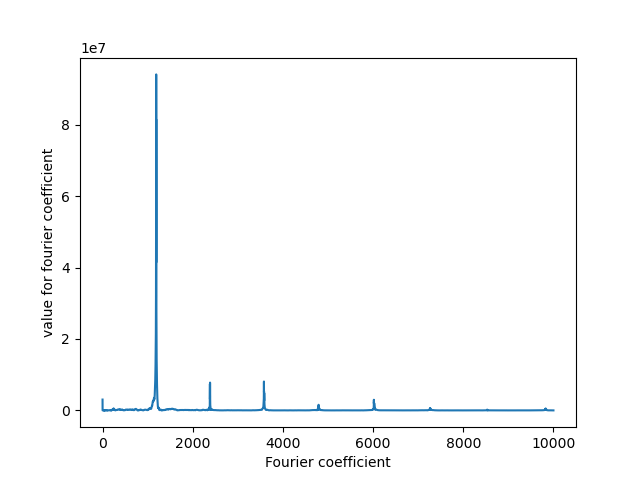
\includegraphics[width=10cm]{8-2-5.png}
\end{table}%

\begin{table}[!h]
    \centering
    \caption{Fourier coefficient for trumpet waveform}
    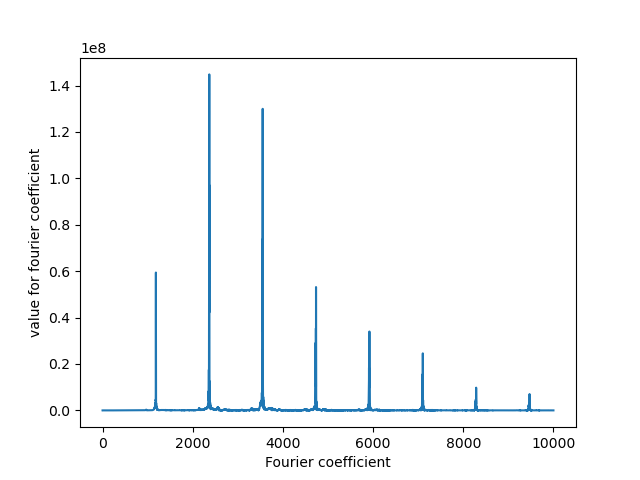
\includegraphics[width=10cm]{8-2-6.png}
\end{table}%
\newpage

From the fourier coefficient, we can see that the waveform of a musical instrument has pretty pure frequency components and low noise. The frequency components are all integer number of a fixed frequency. This can be explained by the nature of stringed instrument, where the resonent frequency of the string is integer number of minimum frequency.

From the fourier coefficient of piano waveform and trumpet waveform, we can find the first peak value. For piano, we found that $n_1 = 1190$ and for trumpet $n_2 = 1184$. We know that the $n^{th}$ fourier coefficient correspond to the waveform:

\begin{equation}
    \phi(i) = e^{i*2\pi*n_i/N}
\end{equation}

Now we know that the data aquisition speed is $f = 44100 Hz$. This means that now for the $n^{th}$ fourier coefficient, the waveform against time is:

\begin{equation}
    \phi(t) = e^{i*2\pi*f*t/N}
\end{equation}

The corresponding frequency is:

\begin{equation}
    f_i = f * n_i/N
\end{equation}

With the total number of data $N = 10^5$, we know that, the frequency of the instrument is:

\begin{itemize}
    \item frequency for piano is 524.79Hz
    \item frequency for trumpet is 522.14Hz
\end{itemize}

We conclude that the musical note it's playing is C5.




\section{Newman 7.4: Fourier filtering and smoothing}

We use numpy to read the txt file into numpy array. This is plotted as follows:

\begin{table}[!h]
    \centering
    \caption{Dow jones industrial index over time}
    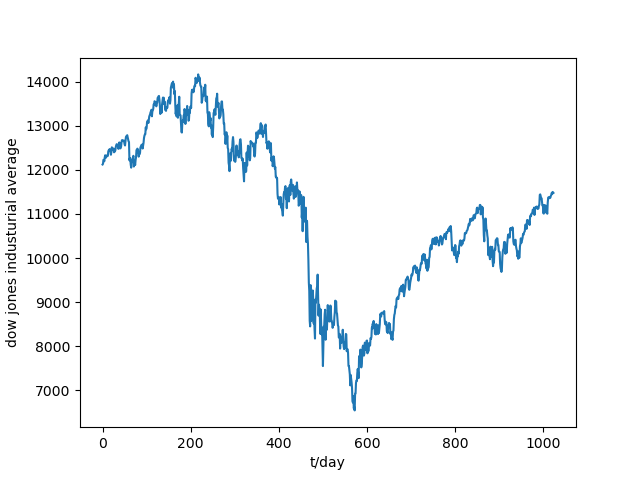
\includegraphics[width=11cm]{8-3-1.png}
\end{table}%
\newpage

We can then do the FFT. We keep the first 10\% of fourier components and do the inverse FFT. The result is plotted below:

\begin{table}[!h]
    \centering
    \caption{Dow jones(original and 10\% smoothed) industrial index over time}
    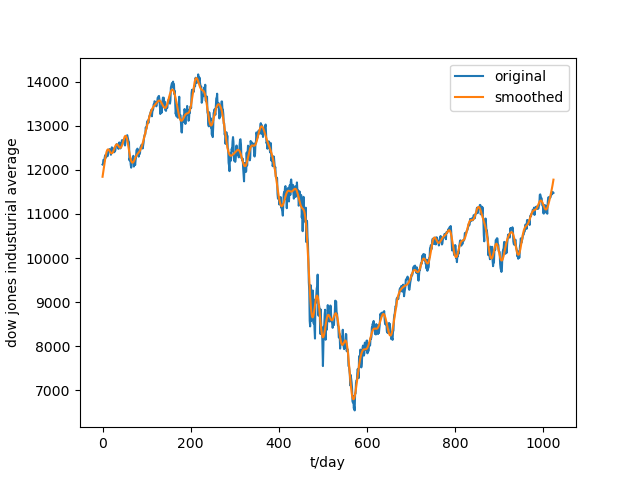
\includegraphics[width=11cm]{8-3-2.png}
\end{table}%
\newpage

We can then do the same thing while only keep first 2\% of the fourier components. The result is plotted below:

\begin{table}[!h]
    \centering
    \caption{Dow jones(original and 2\% smoothed) industrial index over time}
    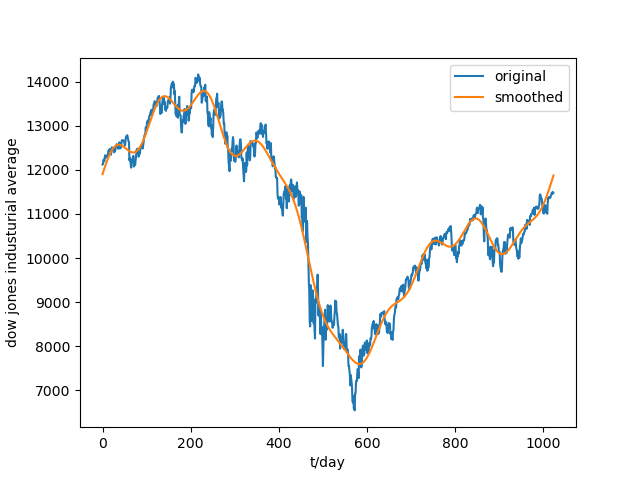
\includegraphics[width=11cm]{8-3-3.png}
\end{table}%
\newpage

We can clearly see that, when we only keep low frequency fourier components, the real curve is smoothed with less short-range detail. The less fourier components we keep, the more the original function is smoothed.


\end{document}